%% ****** Start of file aiptemplate.tex ****** %
%%
%%   This file is part of the files in the distribution of AIP substyles for REVTeX4.
%%   Version 4.1 of 9 October 2009.
%%
%
% This is a template for producing documents for use with 
% the REVTEX 4.1 document class and the AIP substyles.
% 
% Copy this file to another name and then work on that file.
% That way, you always have this original template file to use.

%\documentclass[aip,jap,numerical,preprint]{revtex4-1}
\documentclass[twocolumn,secnumarabic,amssymb, nobibnotes, aps, pra]{revtex4}
\newcommand{\revtex}{REV\TeX\ }
\newcommand{\classoption}[1]{\texttt{#1}}
\newcommand{\macro}[1]{\texttt{\textbackslash#1}}
\newcommand{\m}[1]{\macro{#1}}
\newcommand{\env}[1]{\texttt{#1}}
\setlength{\textheight}{9.5in}

\usepackage{amsmath}
\usepackage{graphicx}
\usepackage{booktabs}
\usepackage{color}
\usepackage{enumerate}
\providecommand{\e}[1]{\ensuremath{\times 10^{#1}}}

%\draft % marks overfull lines with a black rule on the right

\begin{document}

%Title of paper
\title{Frank-Hertz Experiment
% \large{Methods of experimental physics} \\ 
 %\normalsize{PHYS 413}
 }

% repeat the \author .. \affiliation  etc. as needed
% \email, \thanks, \homepage, \altaffiliation all apply to the current
% author. Explanatory text should go in the []'s, actual e-mail
% address or url should go in the {}'s for \email and \homepage.
% Please use the appropriate macro foreach each type of information

% \affiliation command applies to all authors since the last
% \affiliation command. The \affiliation command should follow the
% other information
% \affiliation can be followed by \email, \homepage, \thanks as well.
\author{Jason Morgan}
%\email[]{Your e-mail address}
%\homepage[]{Your web page}
%\thanks{}
%\altaffiliation{}
\affiliation{Department of Physics, Old Dominion University, Norfolk VA 23529}



\date{April 29, 2014}


\begin{abstract}
The purpose of this experiment is to demonstrate the quantized energy levels in electrons. Electrons emitted from a heating element are accelerated through neon gas.  The change in current with respect to applied voltage is measured to find the transitions in neon the neon gas
\end{abstract}

\maketitle
\section{Introduction}

The quantization of energy levels was introduced with the Bohr model of the atom by Neils Bohr in 1913.  The concept was introduced to prevent electron orbits from decaying into the nucleus of the atom due to the emission of electromagnetic radiation that occurs when an electron or other charged particle is accelerated.  An object such as an electron that has an angular velocity is constantly accelerating.  With out the quantization of energy, the atom would be unstable.

Franck Hertz and Gustav Hertz performed the Franl-Hertz experiment to verify this prediction.  They used a vacume tube containing liquid mercury, an anode, a cathode and a heating element to heat the cathode.  Electrons from a heating element were then accelerated through the mercury vapor by an electric potential and the current at the anode was measured.  The electrons traverse the tube and collide with mercury atoms.  These interactions affect the current at the anode.  

The first drop in current at the collector is caused by ellastic collisions between the electrons and mercury atoms.  The second and third drops are caused by inelastic collisions.  The distance between the peaks represent the energy gap between the energy levels in the atoms beign studied.

\section{Experimental setup and procedures}

In this version of the Frank-Hertz experiment, Neon gas is used instead of mercury vapor.  The has the benefits of not needing to heat the vacume tube in an oven to vaporize mercury since Ne is already a gas at room temperature and Ne is not a hadzardous material.  

\begin{figure} [h]  %htb stands for here, top and bottom and gives a suggestion to Latex where to place the graph
\begin{center}
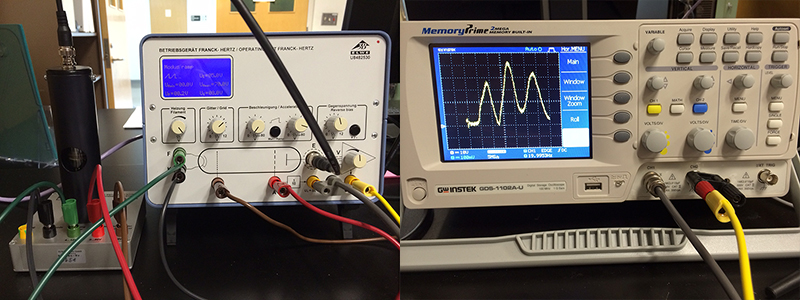
\includegraphics[width=85mm]{setup.jpg} 
\end{center}
\caption{Experiment Setup}
\label{fig:setup}
\end{figure}

The experiment was begun by connecting the equipment with all voltages set to 0V and the power supply unplugged .  The Frank-Hertz tube, and power supply were connected according to the color codes on the connections.  The oscilliscope was connected to the power supply such that is measured the acceleratin voltage on channel one and the anode voltage on channel two.  The scope was then set in X-Y mode so that this data was plotted as anode current vs acceleration voltage (Fig. \ref{fig:setup}).  

\begin{figure} [h]  %htb stands for here, top and bottom and gives a suggestion to Latex where to place the graph
\begin{center}
\includegraphics[width=85mm]{hertzgraphpic.eps} 
\end{center}
\caption{Oscilloscope giving readings in X-Y mode}
\label{fig:pic}
\end{figure}

The power supply was then turned on and the voltage to the heating element was gradually increased until it could be observed to glow.  The element began to glow at 8.2 $\pm$ 0.1 V.  The control grid and and collection anode was set at 8.0 $\pm$ 0.1 V and 5.0  $\pm$ 0.1 V respectively.  The first set of data was then taken with the accelating voltage set to sweep between 0.0 and 70.0  $\pm$ 0.1 V.  After adjusting the gain on the anode, the graph in Fig. \ref{fig:pic} was displayed on the oscilloscope and the data was saved.

\begin{table} [h]  % Capital letters stronger suggestion
\caption{Voltage Separation Between Peaks}      %title of the table     
\centering              % centering table
\begin{tabular}{ccc} % creating four columns (c stands for ceneter, r for right, l for left)
\hline\hline %inserting double-line
  Peak No & Voltage Difference (V)   \\
\hline % inserts single-line
1 & 17 $\pm$ 1   \\
2 & 20 $\pm$ 1  \\
3 & 24 $\pm$ 1  \\
\hline % inserts single-line
\end{tabular}
\label{tab:peaks}
\end{table}

The resulting graph shows three drops in in the current at the anode.  The distance between the peaks was measured using the oscilloscope's cursor functionality and the results are displayed in the table below (Table \ref{tab:peaks}).  This process was then repeated using differing values for the accelerating voltage and heater voltage.  

\section{Results and Discussion}

Neither changing the heater voltage nor the accelerating voltage was observed to alter the distance between the peaks.  Lowering the heater voltage caused a decrease in the amplitude of the wave form and eventually increased the noisy ness of the graph until it was not decernable.  Lowering the accelerating voltage caused the graph to not extend as far, reducing the number of peaks as the maximum accelerating voltage was decreased.  Regardless of the settings it was found that the excitation voltage (distance between peaks) was 20 $\pm$ 1 V.  This is consistent with the expected value of 19V with an error percentage of 5\% 

The wavelength of the emission associated with this transition can now be found using 

Once absorbed, the energy gained by the neon atoms must be re-emitted. The wavelength of this emission can be found using equation \ref{eq:one},:

\begin{equation}
\lambda = \frac{hc}{E},
\label{eq:one}   %label the equation
\end{equation}

 $\lambda$ is the wavelength in meters, h is Planck's constant (4.13\e{-15}) in \textit{e}V-s, c is the speed of light (2.99\e{8}) in m/s and E is the measured energy of 20 V per electron. This gives a wavelength of 62 nm.  




\section{Conclusion}

This experiment was able to reproduce the Franck and Hertz finding that the energy levels of electrons in atoms is guantized confirming Bohr's prediction.  
 
%Using one or two paragraphs, briefly summarize the experiment and describe the key discoveries.  In this section, reasonable suggestions on how to improve the experiment would be helpful.


\begin{figure} [b]  %htb stands for here, top and bottom and gives a suggestion to Latex where to place the graph
\begin{center}
\includegraphics[scale=.5]{frankhertz.pdf} 
\end{center}
\caption{Smoothed X-Y Graph of anode current vs accellerating voltage, the area of the circles represents the error.}
\label{fig:graph}
\end{figure}


%Write down references
%-----------------------------------
\begin{thebibliography}{5}
\bibitem{mcalister1} Wikipedia. "Franck-Hertz Experiment.", \textit{Wikipedia}, Wikimedia Foundation, 03 Sept. 2014. Web. 27 Mar. 2014.
\bibitem{darbas1} M. Nikolić, C. I. Sukenik, \textit{Frank Hertz Experiment with Neon}, (Old Dominion University, Physics 413, 2014).

\end{thebibliography}

\end{document}

%
% ****** End of file aiptemplate.tex ******
